\tikzstyle{block} = [draw, rectangle, minimum height=2em, minimum width=2em,fill=yellow!40!white]
\tikzstyle{sum} = [draw, circle, node distance=1.5cm,fill=yellow!40!white]
\tikzstyle{input} = [coordinate]
\tikzstyle{output} = [coordinate]

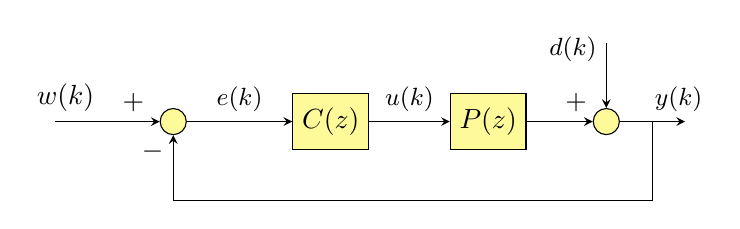
\begin{tikzpicture}[auto,>=stealth]
\node[input] (yo) {};
\node[sum,right of=yo] (sum) {};
\node[block,right of=sum,node distance=2cm] (C) {$C(z)$};
\node[block,right of=C,node distance=2cm] (P) {$P(z)$};
\node[sum,right of=P] (sum2) {};
\node[input,above of=sum2] (d) {};
\node[output,right of=sum2] (y) {};
\node[coordinate,below of=sum] (fb) {};

\draw[->] (yo) -- node[above,pos=0.1]{$w(k)$} node[above,near end]{$+$}(sum);
\draw[->] (sum) -- node[above]{{\small $e(k)$}} (C);
\draw[->] (C) -- node[above]{{\small $u(k)$}} (P);
\draw[->] (P) -- node[above,near end]{$+$} (sum2);
\draw[->] (sum2) -- node(yn){} node[above,pos=0.9]{{\small $y(k)$}} (y);
\draw[->] (d) -- node[left,pos=0.1]{{\small $d(k)$}} (sum2);
\draw[-] (yn) |- (fb);
\draw[->] (fb) -- node[near end]{$-$} (sum);

\end{tikzpicture}
